% Options for packages loaded elsewhere
\PassOptionsToPackage{unicode}{hyperref}
\PassOptionsToPackage{hyphens}{url}
%
\documentclass[
  10pt,
]{article}
\usepackage{amsmath,amssymb}
\usepackage{iftex}
\ifPDFTeX
  \usepackage[T1]{fontenc}
  \usepackage[utf8]{inputenc}
  \usepackage{textcomp} % provide euro and other symbols
\else % if luatex or xetex
  \usepackage{unicode-math} % this also loads fontspec
  \defaultfontfeatures{Scale=MatchLowercase}
  \defaultfontfeatures[\rmfamily]{Ligatures=TeX,Scale=1}
\fi
\usepackage{lmodern}
\ifPDFTeX\else
  % xetex/luatex font selection
  \setmainfont[]{DejaVu Sans}
  \setmonofont[]{DejaVu Sans Mono}
\fi
% Use upquote if available, for straight quotes in verbatim environments
\IfFileExists{upquote.sty}{\usepackage{upquote}}{}
\IfFileExists{microtype.sty}{% use microtype if available
  \usepackage[]{microtype}
  \UseMicrotypeSet[protrusion]{basicmath} % disable protrusion for tt fonts
}{}
\makeatletter
\@ifundefined{KOMAClassName}{% if non-KOMA class
  \IfFileExists{parskip.sty}{%
    \usepackage{parskip}
  }{% else
    \setlength{\parindent}{0pt}
    \setlength{\parskip}{6pt plus 2pt minus 1pt}}
}{% if KOMA class
  \KOMAoptions{parskip=half}}
\makeatother
\usepackage{xcolor}
\usepackage[margin=22mm]{geometry}
\usepackage{color}
\usepackage{fancyvrb}
\newcommand{\VerbBar}{|}
\newcommand{\VERB}{\Verb[commandchars=\\\{\}]}
\DefineVerbatimEnvironment{Highlighting}{Verbatim}{commandchars=\\\{\}}
% Add ',fontsize=\small' for more characters per line
\newenvironment{Shaded}{}{}
\newcommand{\AlertTok}[1]{\textcolor[rgb]{1.00,0.00,0.00}{\textbf{#1}}}
\newcommand{\AnnotationTok}[1]{\textcolor[rgb]{0.38,0.63,0.69}{\textbf{\textit{#1}}}}
\newcommand{\AttributeTok}[1]{\textcolor[rgb]{0.49,0.56,0.16}{#1}}
\newcommand{\BaseNTok}[1]{\textcolor[rgb]{0.25,0.63,0.44}{#1}}
\newcommand{\BuiltInTok}[1]{\textcolor[rgb]{0.00,0.50,0.00}{#1}}
\newcommand{\CharTok}[1]{\textcolor[rgb]{0.25,0.44,0.63}{#1}}
\newcommand{\CommentTok}[1]{\textcolor[rgb]{0.38,0.63,0.69}{\textit{#1}}}
\newcommand{\CommentVarTok}[1]{\textcolor[rgb]{0.38,0.63,0.69}{\textbf{\textit{#1}}}}
\newcommand{\ConstantTok}[1]{\textcolor[rgb]{0.53,0.00,0.00}{#1}}
\newcommand{\ControlFlowTok}[1]{\textcolor[rgb]{0.00,0.44,0.13}{\textbf{#1}}}
\newcommand{\DataTypeTok}[1]{\textcolor[rgb]{0.56,0.13,0.00}{#1}}
\newcommand{\DecValTok}[1]{\textcolor[rgb]{0.25,0.63,0.44}{#1}}
\newcommand{\DocumentationTok}[1]{\textcolor[rgb]{0.73,0.13,0.13}{\textit{#1}}}
\newcommand{\ErrorTok}[1]{\textcolor[rgb]{1.00,0.00,0.00}{\textbf{#1}}}
\newcommand{\ExtensionTok}[1]{#1}
\newcommand{\FloatTok}[1]{\textcolor[rgb]{0.25,0.63,0.44}{#1}}
\newcommand{\FunctionTok}[1]{\textcolor[rgb]{0.02,0.16,0.49}{#1}}
\newcommand{\ImportTok}[1]{\textcolor[rgb]{0.00,0.50,0.00}{\textbf{#1}}}
\newcommand{\InformationTok}[1]{\textcolor[rgb]{0.38,0.63,0.69}{\textbf{\textit{#1}}}}
\newcommand{\KeywordTok}[1]{\textcolor[rgb]{0.00,0.44,0.13}{\textbf{#1}}}
\newcommand{\NormalTok}[1]{#1}
\newcommand{\OperatorTok}[1]{\textcolor[rgb]{0.40,0.40,0.40}{#1}}
\newcommand{\OtherTok}[1]{\textcolor[rgb]{0.00,0.44,0.13}{#1}}
\newcommand{\PreprocessorTok}[1]{\textcolor[rgb]{0.74,0.48,0.00}{#1}}
\newcommand{\RegionMarkerTok}[1]{#1}
\newcommand{\SpecialCharTok}[1]{\textcolor[rgb]{0.25,0.44,0.63}{#1}}
\newcommand{\SpecialStringTok}[1]{\textcolor[rgb]{0.73,0.40,0.53}{#1}}
\newcommand{\StringTok}[1]{\textcolor[rgb]{0.25,0.44,0.63}{#1}}
\newcommand{\VariableTok}[1]{\textcolor[rgb]{0.10,0.09,0.49}{#1}}
\newcommand{\VerbatimStringTok}[1]{\textcolor[rgb]{0.25,0.44,0.63}{#1}}
\newcommand{\WarningTok}[1]{\textcolor[rgb]{0.38,0.63,0.69}{\textbf{\textit{#1}}}}
\usepackage{graphicx}
\makeatletter
\def\maxwidth{\ifdim\Gin@nat@width>\linewidth\linewidth\else\Gin@nat@width\fi}
\def\maxheight{\ifdim\Gin@nat@height>\textheight\textheight\else\Gin@nat@height\fi}
\makeatother
% Scale images if necessary, so that they will not overflow the page
% margins by default, and it is still possible to overwrite the defaults
% using explicit options in \includegraphics[width, height, ...]{}
\setkeys{Gin}{width=\maxwidth,height=\maxheight,keepaspectratio}
% Set default figure placement to htbp
\makeatletter
\def\fps@figure{htbp}
\makeatother
\setlength{\emergencystretch}{3em} % prevent overfull lines
\providecommand{\tightlist}{%
  \setlength{\itemsep}{0pt}\setlength{\parskip}{0pt}}
\setcounter{secnumdepth}{-\maxdimen} % remove section numbering
\ifLuaTeX
  \usepackage{selnolig}  % disable illegal ligatures
\fi
\usepackage{bookmark}
\IfFileExists{xurl.sty}{\usepackage{xurl}}{} % add URL line breaks if available
\urlstyle{same}
\hypersetup{
  hidelinks,
  pdfcreator={LaTeX via pandoc}}

\author{}
\date{}

\begin{document}

\section{DDTA Documentation Metamodel Through Functional Requirement -
Closure Checkpoint
R2}\label{ddta-documentation-metamodel-through-functional-requirement---closure-checkpoint-r2}

\textbf{THESIS BASELINE CHECKPOINT}

\subsection{1. Evidence rule}\label{1-evidence-rule}

This checkpoint intentionally \textbf{excludes} the two earlier
oversimplified order/inventory holdouts and the earlier facial direct-MR
FR probes as evidence for hierarchy. Those examples embedded choices
inside MR/FR prose or simplified domain responsibilities enough to bias
the topology result.

The current hierarchy conclusion is based on the corrected
access-control reasoning plus the realistic order/warehouse rewrite in
\texttt{../03-example-order-fulfillment/ORDER\_FULFILLMENT\_COMPLETE\_AUTHORING\_PROBE\_R3.*}.

\subsection{2. Closed documentation hierarchy for thesis
scope}\label{2-closed-documentation-hierarchy-for-thesis-scope}

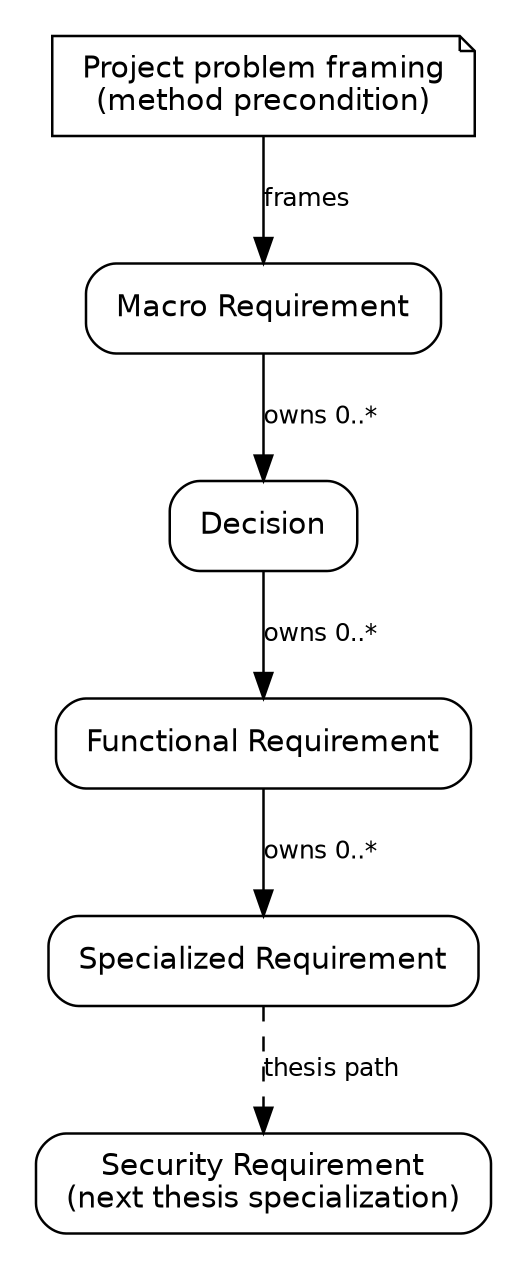
\includegraphics{diagrams/DOCUMENT_HIERARCHY.png}

\begin{Shaded}
\begin{Highlighting}[]
\NormalTok{Project problem framing        [method precondition, not governed document]}
\NormalTok{        |}
\NormalTok{        v}
\NormalTok{MacroRequirement}
\NormalTok{        |}
\NormalTok{        v}
\NormalTok{Decision}
\NormalTok{        |}
\NormalTok{        v}
\NormalTok{FunctionalRequirement}
\NormalTok{        |}
\NormalTok{        v}
\NormalTok{SpecializedRequirement}
\NormalTok{        |}
\NormalTok{        \textasciigrave{}{-}{-} SecurityRequirement   [next specialization to formalize]}
\end{Highlighting}
\end{Shaded}

Cardinality/lifecycle interpretation:

\begin{itemize}
\tightlist
\item
  an MR may exist before Decisions are authored;
\item
  every Decision has exactly one MR parent;
\item
  every FR has exactly one Decision parent;
\item
  a Decision may exist before FR children are authored;
\item
  no FR has a direct MR parent in the thesis baseline;
\item
  no Decision is a child of FR;
\item
  an FR may later own \texttt{0..*} Specialized Requirements.
\end{itemize}

\subsection{3. Why keep the Decision layer
constant}\label{3-why-keep-the-decision-layer-constant}

Across access-control and warehouse examples, apparently "direct" FRs
repeatedly concealed a prior commitment:

\begin{itemize}
\tightlist
\item
  facial verification required choosing the verification
  modality/responsibility;
\item
  biometric/reference management required choosing the source/authority
  boundary;
\item
  warehouse receipt/reservation behavior required deciding whether stock
  is project-managed or delegated to an external WMS;
\item
  payment behavior changed when processing was delegated to an external
  PSP.
\end{itemize}

The regular layer makes these commitments explicit and simplifies
authoring, validation, navigation and tooling.

\subsubsection{Rare singleton-solution
trade-off}\label{rare-singleton-solution-trade-off}

The model accepts a controlled \textbf{necessity/default Decision} when
no materially distinct admissible alternative exists. This is an
intentional methodological normalization: the project documents the
commitment and why the alternative set is singleton rather than varying
the hierarchy.

The rule is not permission to invent false rationale. Context must show
why alternatives are absent/excluded, Consequences must be material, and
the Decision must be reopenable if the constraint changes.

\subsection{4. Closed MR semantics}\label{4-closed-mr-semantics}

MR owns one stable macro responsibility inside the framed problem.

Key invariants:

\begin{itemize}
\tightlist
\item
  problem anchored;
\item
  one coherent macro concern;
\item
  architecture/temporal resilience;
\item
  no solution commitment leakage;
\item
  no atomic FR behavior;
\item
  broad domain readability;
\item
  explicit cross-MR dependency;
\item
  teachability;
\item
  analysis-enabling, not analysis-producing.
\end{itemize}

Fundamental question:

\begin{quote}
Within the framed project problem, which stable macro responsibility are
we governing, what macro result/value must it contribute, why does it
matter, and who is involved?
\end{quote}

\subsection{5. Closed Decision
semantics}\label{5-closed-decision-semantics}

Decision owns one significant commitment narrowing one MR.

Local core:

\begin{Shaded}
\begin{Highlighting}[]
\NormalTok{Decision}
\NormalTok{|{-} title}
\NormalTok{|{-} context}
\NormalTok{|{-} decision}
\NormalTok{\textasciigrave{}{-} consequences}
\end{Highlighting}
\end{Shaded}

Normally it selects among alternatives; exceptionally it records a
necessity/default commitment when the admissible alternative space is
singleton after review.

\subsection{6. Closed FR semantics}\label{6-closed-fr-semantics}

FR is an independently assessable operational obligation under one
parent Decision.

It contains:

\begin{itemize}
\tightlist
\item
  one coherent functional obligation;
\item
  one or more readable normative clauses;
\item
  structured SPO references supporting those clauses;
\item
  exactly one parent Decision.
\end{itemize}

Normative prose is primary; SPO does not replace
conditional/concurrency/lifecycle/failure semantics.

\subsection{7. Cross-MR service
composition}\label{7-cross-mr-service-composition}

The semantic rule is closed:

\begin{quote}
A consumer branch may use a governed service/capability owned by another
MR without transferring ownership or creating a second parent.
\end{quote}

The exact L1 target of that consumption relation is \textbf{not} closed
yet. It will be decided with Base Analysis because the natural target
may be a service/capability/BAE/interface rather than one specific FR.

\subsection{8. What remains deliberately
open}\label{8-what-remains-deliberately-open}

The closure does not yet formalize:

\begin{itemize}
\tightlist
\item
  Base Analysis / BAE types, relations, provenance and incremental
  creation from governed documentation;
\item
  formal service/capability representation between MR branches;
\item
  overlay/plugin contract;
\item
  Analysis Record and Common Finding integration;
\item
  SecurityRequirement fields/cardinalities/provenance from accepted
  Finding;
\item
  effective obligation construction
  (\texttt{FR\ +\ applicable\ SecurityRequirement});
\item
  canonical L2 Markdown/YAML encoding beyond the authoring contract;
\item
  realization/verification evidence lifecycle.
\end{itemize}

\subsection{9. Reopen conditions}\label{9-reopen-conditions}

Reopen MR/Decision/FR semantics only if a concrete later result
demonstrates that:

\begin{enumerate}
\def\labelenumi{\arabic{enumi}.}
\tightlist
\item
  a SecurityRequirement cannot correctly constrain an FR under this
  hierarchy;
\item
  Base Analysis cannot be built/integrated from governed documentation
  without requiring different document semantics;
\item
  a method overlay requires source information the authoring model
  cannot express without contaminating MR/Decision/FR with
  method-specific concepts;
\item
  the regular Decision layer creates a concrete recurring semantic
  failure rather than merely an extra rare normalization document.
\end{enumerate}

\subsection{10. Authorized next phase}\label{10-authorized-next-phase}

\begin{Shaded}
\begin{Highlighting}[]
\NormalTok{fixed documentation authoring}
\NormalTok{        |}
\NormalTok{        v}
\NormalTok{formal Base Analysis / BAE}
\NormalTok{        |}
\NormalTok{        v}
\NormalTok{method{-}neutral overlay contract}
\NormalTok{        |}
\NormalTok{        v}
\NormalTok{STRIDE plugin/overlay as first concrete test}
\NormalTok{        |}
\NormalTok{        v}
\NormalTok{Analysis Record {-}\textgreater{} reviewed Finding}
\NormalTok{        |}
\NormalTok{        v}
\NormalTok{SecurityRequirement}
\NormalTok{        |}
\NormalTok{        v}
\NormalTok{FR + SEC effective obligation}
\NormalTok{        |}
\NormalTok{        v}
\NormalTok{revised design {-}\textgreater{} re{-}analysis}
\end{Highlighting}
\end{Shaded}

The purpose of the next phase is to verify the entire DDTA loop, not
merely to prove that an overlay can emit threat labels.

\end{document}
